\section{Regular expressions and FSA}

Consider the regular expression $R$ below, over the three-letter alphabet $\Sigma=\{a,b,c\}$ 
\[R=a\left( b|c^{+}a \right)^{*}\]
Answer the following questions:
\begin{enumerate}
    \item Write all the strings $x$ of the language of $R$ that have a length less than or equal to four, i.e., $x \in L(R)$ with $|x| \leq 4$, in lexicographic order (with $a < b < c$).
    \item By means of the Berry-Sethi method, find a deterministic automaton $A$ equivalent to the regular expression $R$. 
    \item Is the deterministic automaton $A$ found before minimal? Justify your answer.
    \item By means of the Brzozowski method (node elimination), starting from the automaton $A$ found before, obtain a regular expression $R^{'}$ equivalent to $A$.
    \item Is the language $L(R)$ locally testable? Formally prove your answer.
\end{enumerate}

\paragraph*{Solution}
\begin{enumerate}
    \item The possible strings include: $a$, $ab$, $abb$, $aca$, $abba$, $abca$, $acab$, $acca$. 
    \item Firstly, we enumerate the symbols for $R_{\#}=a_1\left( b_2|c^{+}_{3}a_4 \right)^{*}\dashv$. 
        We construct the following support table:
        \begin{table}[H]
            \centering
            \begin{tabular}{cc}
            Initials                       & $a_1$             \\ \hline
            \multicolumn{1}{c|}{Terminals} & Followers         \\
            \multicolumn{1}{c|}{$a_1$}     & $b_2c_3\dashv$ \\
            \multicolumn{1}{c|}{$b_2$}     & $b_2c_3\dashv$  \\
            \multicolumn{1}{c|}{$c_3$}     & $c_3a_4$         \\
            \multicolumn{1}{c|}{$a_4$}     & $b_2c_3\dashv$ 
            \end{tabular}
        \end{table}
        We begin with the initial state and proceed as follows:
        \begin{figure}[H]
            \centering
            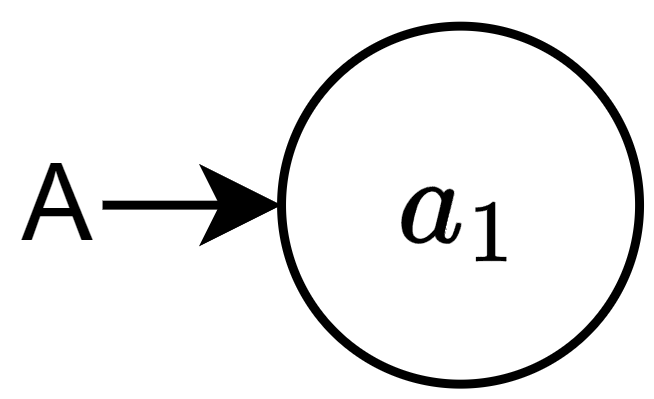
\includegraphics[width=0.2\linewidth]{images/FSA1.png}
        \end{figure}
        Next, we create a state reachable from $a_1$, resulting in:
        \begin{figure}[H]
            \centering
            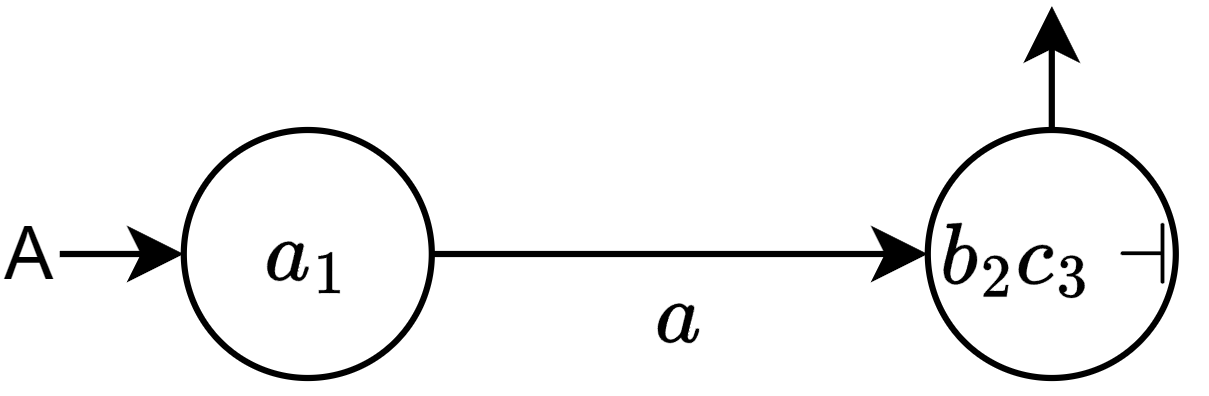
\includegraphics[width=0.4\linewidth]{images/FSA2.png}
        \end{figure}
        After performing these steps for all states, we obtain the following automaton:
        \begin{figure}[H]
            \centering
            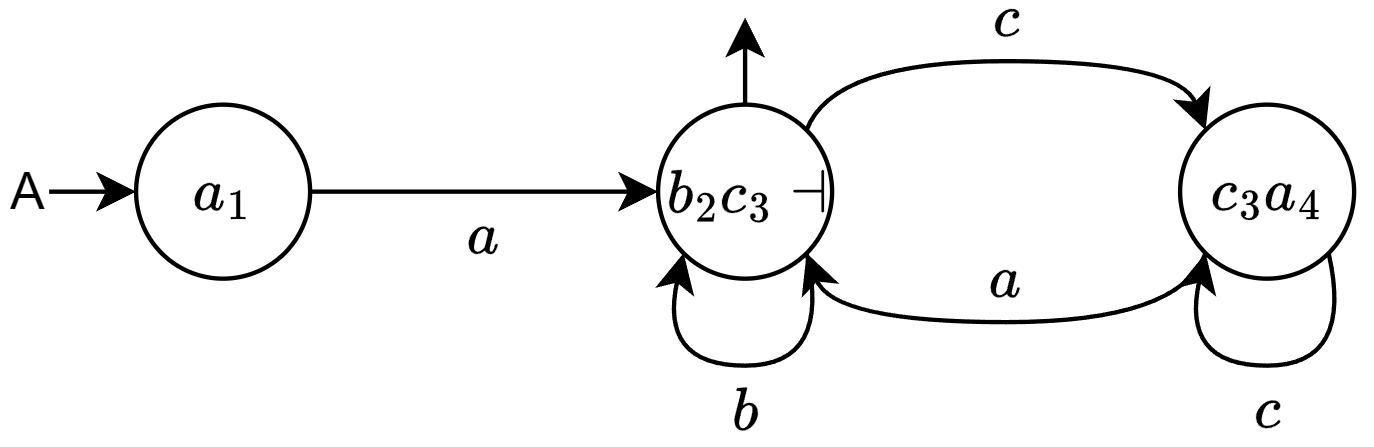
\includegraphics[width=0.5\linewidth]{images/FSA3.png}
        \end{figure}
    \item Automaton reduction involves minimizing the number of states.
        To simplify the automaton, we start by renaming the states:
        \begin{figure}[H]
            \centering
            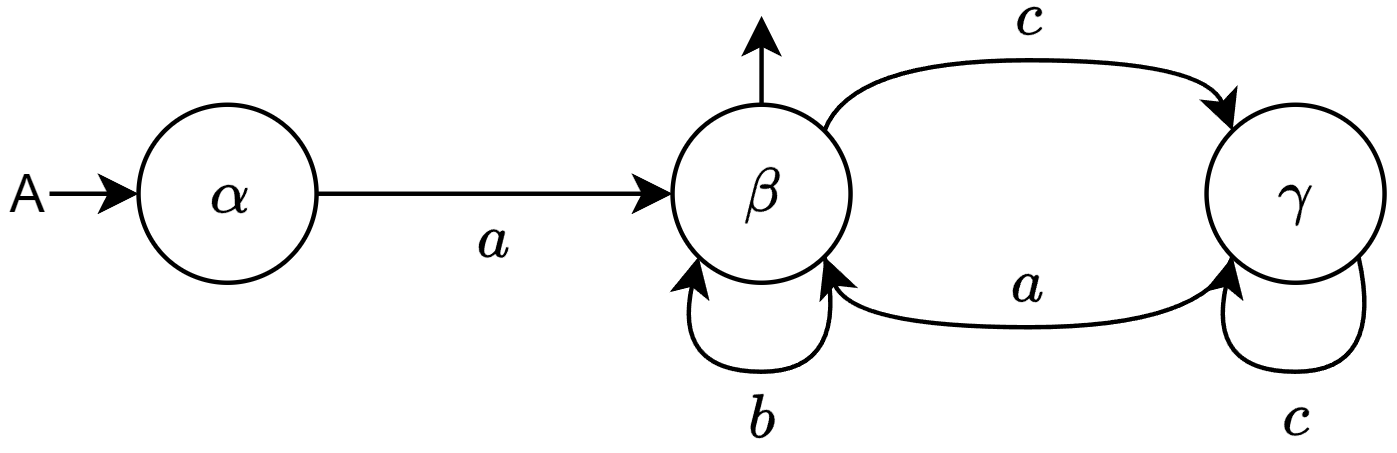
\includegraphics[width=0.5\linewidth]{images/FSA4.png}
        \end{figure}
        We observe that $\alpha$ cannot be merged with $\beta$ due to one being final and the other not. 
        The same holds for $\beta$ and $\gamma$. 
        States $\alpha$ and $\gamma$ cannot be merged due to differing transitions.
        Thus, the three states are distinguishable, and the automaton is minimal.
    \item We begin by creating a virtual initial and final node connected to the automaton:
        \begin{figure}[H]
            \centering
            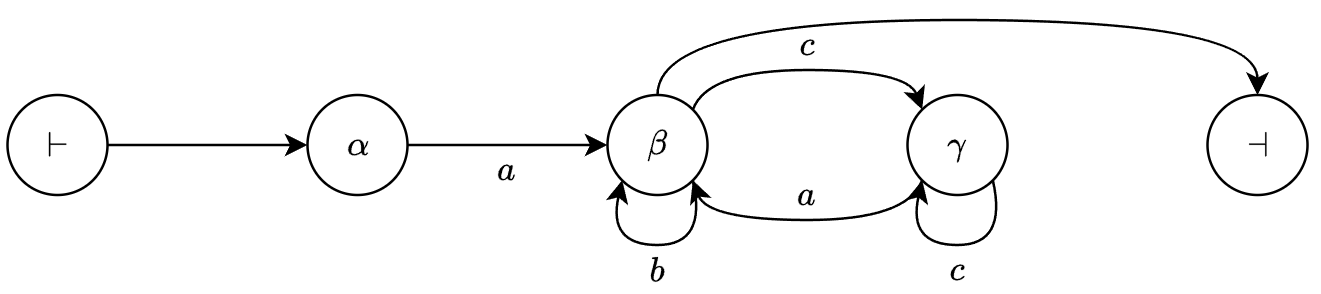
\includegraphics[width=0.75\linewidth]{images/FSA5.png}
        \end{figure}
        We then remove states one by one until reaching the final state directly from the initial one. 
        We start by removing $\gamma$ with the loop $c^{+}a$. 
        We have two cycles on $\beta$ that can be substituted with the expression $(b|c^{+}a)^{*}$. 
        The only state remaining is $\alpha$, and we finally have: 
        \[R^{'}=a(b|c^{+}a)^{*}\]
    \item The sets are as follows:
        \begin{itemize}
            \item Initials: $\{a\}$
            \item Finals: $\{a,b\}$
            \item Digrams: $\{aa,ac,bb,bc,ca,cc\}$
        \end{itemize}
        Using these sets, we construct a specific automaton $A^{'}$. 
        The initial set is connected to the set of initials, the final states are those in the finals set, and the transitions are based on the digrams set.
        \begin{figure}[H]
            \centering
            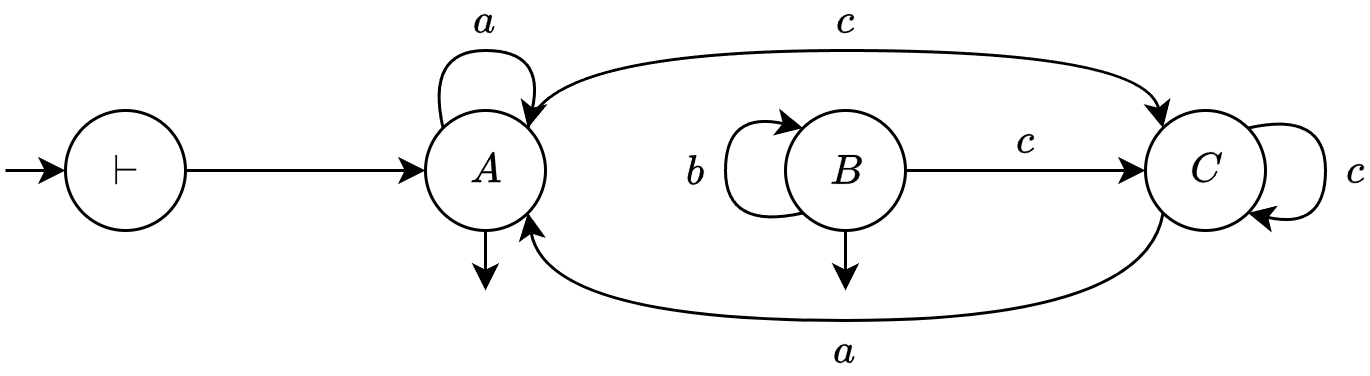
\includegraphics[width=0.75\linewidth]{images/FSA6.png}
        \end{figure}
        The automaton is locally testable if it recognizes the initial language, and the edge reached by an arc has the same name as the transition.
        In this case, we constructed the nodes such that the second property is satisfied.
        We observe that states $a$ and $b$ are not distinguishable, allowing us to reduce the automaton to $A$. 
        Therefore, the language is locally testable.
\end{enumerate}